\section{Theorie}
\label{sec:Theorie}

Das Elastizitätsmodul $E$ beschreibt die physikalische Materialkonstante,
die als Proportionalitätskonstante im Hookschen Gesetz vorkommt.
Es ist also eine maßgebliche Einheit, für die Elastizität eines Objektes.
Das \textbf{Hookesche Gesetz} lautet
\begin{equation}
        \sigma = E \cdot \frac {\increment L}{L} \text{ ,}
\end{equation}
wobei $\frac {\increment L}{L}$ die relative Änderung einer Körperdimension beschreibt.
Anschaulich ist dies in Abbildung \ref{fig:Hook1} dargestellt.

\begin{figure}[H]
        \centering
        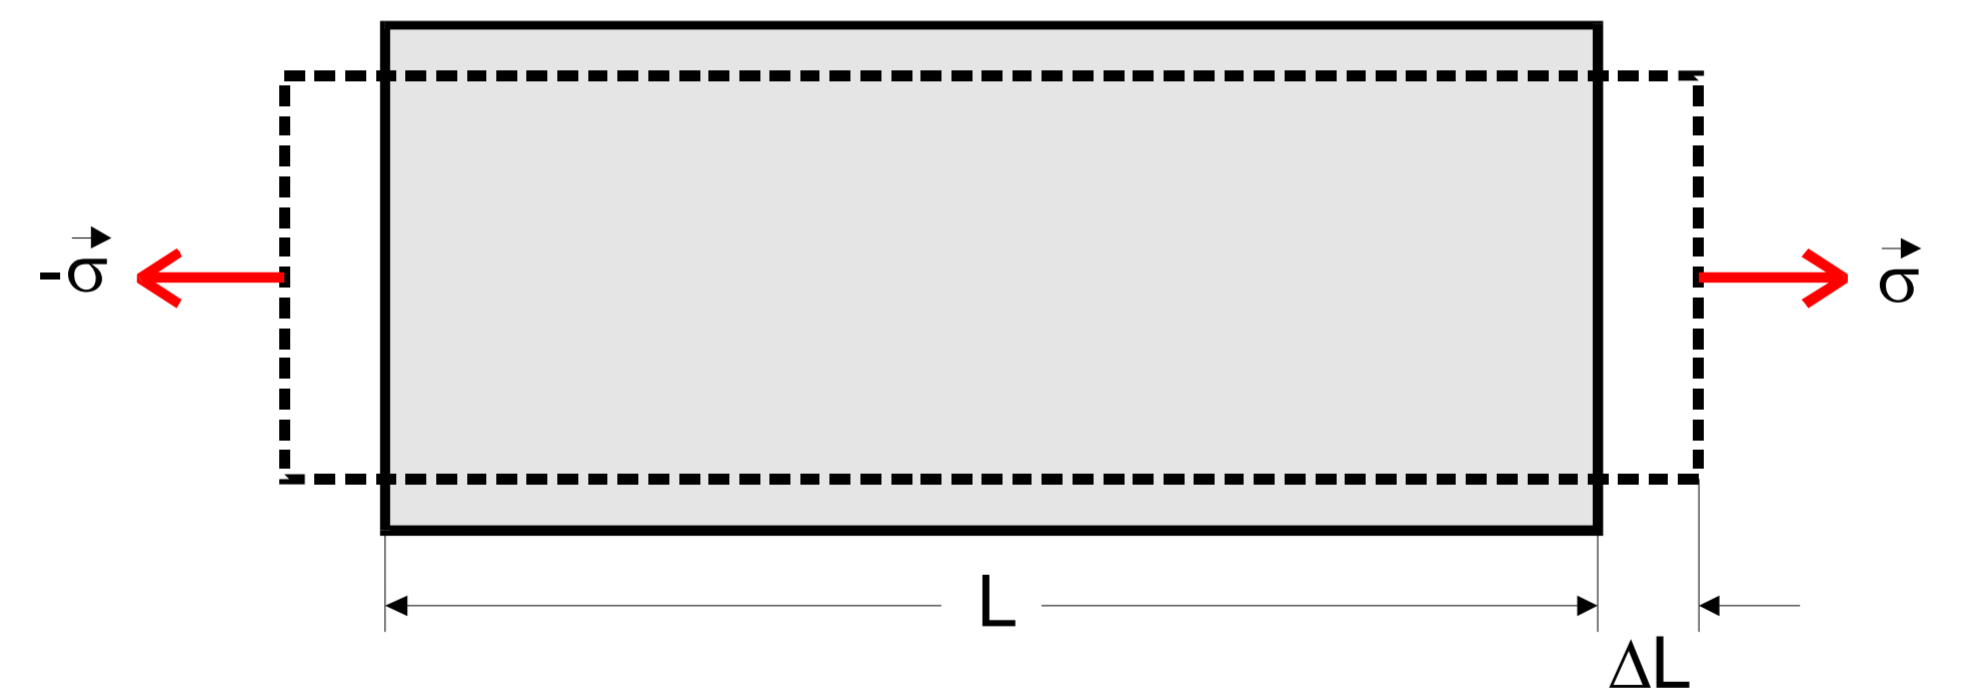
\includegraphics[width=\textwidth]{pictures/Hook1.png}
        \caption{Darstellung des Hookeschen Gesetztes.}
        \label{fig:Hook1}
\end{figure}

Um schließlich $E$ zu bestimmen, werden in diesem Versuch Metallstäbe unbekannten Materials eingespannt und die Biegung untersucht.
Die Biegung entsteht durch ein angehängtes Gewicht an das Ende des Stabes.
Dieses sorgt durch die Gravitation für ein \textit{äußeres} Drehmoment auf den Stab.
Dieses Drehmoment lässt den Stab biegen, jedoch nur bis zu dem Punkt, an dem das \textit{innere} Drehmoment dem äußeren entspricht.
% Werden nun die Formel für das jeweilige Moment gleichgesetzt, ergibt sich
% \begin{equation}
%         \int_\text{Q} y \sigma(y) dq = F (L - x) \text{ ,}
% \end{equation}
% wobei $\sigma(y)$ die Normalspannung und y den Abstand zur neutralen Faser $x$ beschreibt.  
Nach Umstellen einiger Formeln, erhält man eine Formel für die Auslenkung $D(x)$.
Es gilt
\begin{equation} \label{eq:E1}
        D(x) = \frac{m \cdot g}{2 E I} (Lx^2 - \frac{x^3}{3}) \text{ .}
\end{equation}
Die beteiligten Größen entsprechen ihren normalen physikalischen Größen.
Das $I$ jedoch beschreibt das sogenannte \textit{Flächenträgheitsmoment}.
Dieses berechnet sich über die Formel
\begin{equation}
        I \coloneq \int_Q y^2 dq(y) \text{ .}
\end{equation}

Das Flächenträgheitsmoment eines Kreises entspricht
\begin{equation}\label{eq:FlTreagKreis}
        I_\text{Kreis} = \int_\text{A} r^2 \cdot dA = \int_0^R 2 \pi r^3 \cdot dr = \frac{R^4 \pi}{2}\text{ .}
\end{equation}

Außerdem für Stäbe mit quadratischem Querschnitt ist das Flächenträgheitsmoment eines Quadrates relevant.
Mit $a = h / 2$ ergibt sich
\begin{equation}\label{eq:FlTreagQuadrat}
        I_\text{Quadrat} = \int_\text{A} a^2 \cdot dA = \frac{h^4} {12} \text{ ,}
\end{equation}
wobei $h$ die Kantenlänge ist.%

Zusätzlich relevant ist die Formel für $D(x)$, wenn beide Enden des Stabes eingespannt werden und
ein Gewicht in die Mitte gehängt wird.
Für diesen Fall ist
\begin{equation} \label{eq:E2}
        D(x) = \frac{m \cdot g}{48 E I} (3L^2x - 4 x^3)
\end{equation}
für $ x \in [0,L/2]$.